\documentclass[nobib]{tufte-handout}

\usepackage{epigraph}
\usepackage{csquotes}
\usepackage{xcolor}
\usepackage{graphicx}
\usepackage{todonotes}
\makeatletter
\renewcommand{\subsubsection}{\ttl@straightclass{subsubsection}}
\makeatother
\titleformat{\subsubsection}[hang]
  {\selectfont\it}
  {\thesubsubsection}
  {1em}
  {}
  []
\newcommand{\placeholdertext}[1]{
	\noindent{\color{red}{#1}}
}

\newcommand{\CiteThis}{
({\color{red}{CITE THIS}})
}

\newcommand{\csharp}{C\# }
\usepackage{lipsum}
\title{Literature Review of Leading Research in Compiler Optimizations}
\author{Timothy Van Slyke}
\begin{document}
\maketitle
\section*{Abstract}
\begin{abstract}
We explore literature from leading researchers in the field of optimizating compilers.  We find a significant portion of research in compiler optimizations targets problems with memory latency, with particular attention being given to improvements in efficient usage of CPU caches.  We additionally observe a trend towards the adoption of dynamic run-time optimization methods.  Aggressive just-in-time compilation strategies are proposed by several researchers as well as several unconvention methods of code generation and transformation in non-JIT contexts.  Additional research appears to be fairly specialized; particularly notable are advancements in polyhedral compilation and automatic parallelization.  We find that many of the methods are orthogonal and mutually comlementary, and observe promising potential in general.
\end{abstract}

\section*{}
% \begin{displayquote}
\noindent{\large \textit{``Software is getting slower more rapidly than hardware becomes faster.''}}
\newline\noindent\hfill{-- Niklaus Wirth} \\
% \end{displayquote}
%%% Introduction %%%
\section{Introduction}
The modern software ecosystem is rich with a variety of platforms with distinct needs.  With the advent of mobile computing\footnote{Here we use the term ``mobile computing/platforms/devices'' to primarily refer to so-called ``smart devices'' such as smart phones and tablets.  While traditional mobile computing devices (i.e. laptops) face many of the same issues as smart devices, they share a fair number of similarities with desktop computers and may not appropriately be described by some of the generalizations discussed here.}, traditional software development practices have seen major disruptions over the past decade.  While the x86 architecture continues to dominate the desktop market, mobile platforms have largely adopted RISC\footnote{Reduced instruction set computer.} architectures; ARM-based CPUs are ubiquitous across all major mobile platforms.  Additionally, the widespread and international usage of social media platforms, web search engines, and other large-scale web services has necessitated an expanding usage of centralized data centers, or ``server farms''.  Both of these platforms, mobile devices and servers, despite having distinctly disparate use cases, make nearly identical demands from the software that they use.

To quote Chandler Carruth, technical lead for Google's C++ and LLVM teams, ``The only thing [a data center does] is take electricity and turn it into heat.  That is its job.'' \cite{Carruth}.  Maintenance of large-scale data centers present some of the largest expenses for firms such as Google, Amazon, Facebook, and other tech giants.  Improvements to the power usage of the software that runs on these servers present a major opportunity for engineers to reduce expenditures.  Similarly, mobile devices are constrained by the fact that they must employ a depletable power source.  Devices which are battery-operated also incentivize low power consumption, by necessity.

To date, the most effective strategy for reducing power consumption by computation has been to increase software speed \cite{Carruth}.  CPUs have developed an impressive capacity for reducing energy usage through selective hibernation.  Modern advice in the software development community for increasing so called ``compute per Watt'' is to ``finish quickly so the device can go to sleep''.

Motivations for producing faster software are plentiful even when ignoring the energy consumption argument.  It would be hard to conceive of a scenario in which making a computer program slower is desired, and certainly such a task could not be difficult to achieve\footnote{It might be argued by some that the task of producing slower programs is a solved problem in modern software development.}.  In light of this universal need for faster software we seek to answer the following question:

\begin{displayquote}
What advancements in the state-of-the-art for compiler optimizations are being pursued in contemporary research?
\end{displayquote}




%% Background %%
\subsection{Background}
Modern optimizing compilers statically-typed programming languages have seen decades maturation.  At a bare minimum, any serious optimizing compiler can be expected to be capable of at least the following:
\begin{itemize}
\item Callsight-sensitive subroutine inlining.
\item Devirtualization. 
\item Copy elision.
\item Loop unrolling. 
\item Target-specific code generation.  
\item Common subexpression elimination.
\item Constant folding.
\item Primitive alias analysis. 
\item Dead code elimination.
\item Register allocation.
\end{itemize}

The above list is, of course, non-exhaustive.  The onus of producing fast computer programs without sacrificing code quality is indeed on compilers alone.  Popular open-source compilers are subject to a high degree of scrutiny due to their widespread adoption by both industry professionals and hobbyists alike.  The GNU Compiler Collection (GCC - originally the GNU C Compiler) and Clang are two primary targets of innovations in the C and C++ programming communities.  The LLVM compiler framework (Clang's parent project) is particularly popular as a platform for experimentation; many of the publications we discuss in this document choose to implement their experiments using LLVM's facilities.

The literature we discuss primarily references compilation strategies for C, C++, and Java.  It is important to note that the compiler ecosystems for C and C++ are largely the same; nearly every modern compiler for either language supports the other\footnote{A minor exception to this rule is Microsoft's Visual C++ Compiler (MSVC), which no longer actively supports C (but can still compile most standards-compliant C99 code).}.  The Java compiler ecosystem is largely a different beast however, due to the fact that Java compilers do no compile to native machine code but instead to virtual machine (VM) bytecode.  Additionally, Java and similar managed languages like \csharp also typically run on a virtual machine with a built-in Just-In-Time (JIT) compiler system.  

It is also worth noting that these compilers must optimize for entirely different object models.  The C and C++ ISO standards specify an object model that necessitates data being stored densely and in-place.  Java (and \csharp), on the other hand, requires exactly the opposite: non-primitive objects are always stored indirectly through an implicit pointer to heap storage.  This has major ramifications for performance; dense data storage promotes cache-locality and thus better memory latency while also making alias analysis more manageable.

\begin{figure}
\centering
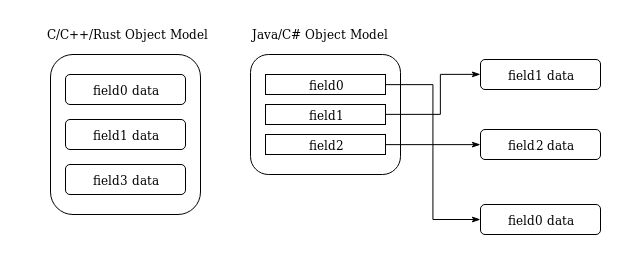
\includegraphics[width=\linewidth]{images/SideBySideObjectModel.png}
\caption{Side-by-side visualization of the C/C++/Rust object model versus the Java/C\# object model.  The C object model promotes densely-stored data and requires aliasing to be expressed through the type system explicitly (via pointers).  This makes compile-time alias analysis tractable and promotes cache-friendly organization of data.\newline The Java object model requires at least one indirection (implicit pointer dereference) to access non-primitive data at run-time and promotes liberal object aliasing through simple pointer copies (reference semantics).  This hinders a compiler's ability to perform alias analysis and hurts cache efficiency by storing objects sparsely.}
\end{figure}



Our discussion will include innovations within the context of both ecosystems.  In particular, we explore the following major trends in modern compiler optimization research, as they relate to both ecosystems:
\begin{itemize}
\item Non-trivial code generation aimed at adaptive run-time performance improvements.
\item State-of-the-art in ``traditional'' optimizations (local code improvements, instruction reordering, static analysis).
\item Automatic parallelization.
\item Improvements to internal modeling methods and algorithms.
\end{itemize}



%% Methods %%
\subsection{Methods}
Optimizing compilers have been the subject of rigorous scrutiny for decades.  Many prominent organizations, particularly firms whose income is reliant on providing software services, have a vested interest in producing software that is reliably fast and efficient modern computer hardware.  As a consequence, a very rich set of compiler optimizations have largely been ``done to death'', so to speak.  To obtain information on the state-of-the-art in this field, we explore publications from a small number of specialized conferences: 
\begin{itemize}
\item Symposium on Principles of Programming Languages
\item Programming Language Design and Implementation (previously Symposium on Compiler Optimization)
\item International Symposium on Code Generation and Optimization
\end{itemize}

With few exceptions, the publications we analyze provide concrete implementations of their respective proposals; we have have chosen to exclude \emph{most} pure compiler theory research from our review.  We analyze optimization intended for traditional compilers, while also exploring specialized techniques like polyhedral compiler systems, the most prominent example of which is PLuTo \cite{Pluto}.  


%%% Modern Compiler Optimizations %%%
\section{Modern Compiler Optimizations}


\subsection{Dynamic Run-time Solutions}
A common roadblock to many compiler optimizations is a lack of information at compile-time.  Certain information can only be known at run-time, for example: 
\begin{itemize}
\item The likelihood that a given conditional branch path will be taken.\footnote{Likely branches are typically called ``hot paths''.}
\item Type information contained in dynamic libraries.
\item Buffer and dynamic array sizes.
\end{itemize}

This lack of information prevents compilers from making informed decisions about how local optimizations should be structured.  Managed languages like Java and \csharp have a built-in opportunity to leverage this information in the form of state-of-the-art JIT compiler techniques.  Languages which require a virtual machine bytecode interpreter typically provide JITs to improve performance by providing facilities to transform VM bytecode to machine code.  Compilers for specific VM run-time environments can implement efficient run-time facilities for dynamic code transformations since they ``own'' both the compiler and the VM.  This enables a larger class of optimizations for compilers because they can operate under the assumption that the unknown information can be collected at run-time.

Languages which are typically compiled directly to machine code (prominent examples being C, C++, and Rust) cannot make the same assumptions as managed languages.  Implementing such facilities would require inserting code for data collection and the corresponding conditional code transformations without support from the run-time environment.  Additionally, and perhaps more importantly, such aggressive transformations are atypical and violate programmers' expectations about code generation.  

Nonetheless, research is being done in this area for both managed and unmanaged programming languages.  This research can largely be categorized into one of the following two categories:
\begin{itemize}
\item Extending existing run-time JIT compilation techniques with new methods.
\item Significant code generation to collect information and dynamically adapt, drastically transforming the behavior of the input source code.
\end{itemize}

\subsubsection{Innovations in JIT Compilers}
Dissegna et al., from Microsoft Research, propose a framework for abstract interpretation in a tracing JIT compiler\cite{Dissegna}.  Their contribution is largely theoretical, but provides a formal means for developing a JIT which can make more liberal run-time modifications to code without introducing ill-formed constructs.  Their framework is the first to successfully describe a JIT that can perform abstract interpretation at run-time.  

More concrete innovations are proposed by Rompf et al., who contribute a framework and corresponding implementation of an API which exposes control of JIT behavior to user code \cite{Rompf}.  Historically, JIT activity has been regarded as an implementation detail of the VM run-time environments.  By allowing user code to steer JIT behavior through the use of a macro system, Rompf et al. were able to observe up to 52$\times$ speed improvements over the default.  Perhaps more significantly, when paired with GPU utilization, their implementation was able to out-perform optimized C++ machine code by a factor of over 2$\times$\cite{Rompf}. 

This development shows significant potential for JIT macro systems. The exposure of compiler internals to the programmer is unorthodox indeed; primary challenges with this technique stem from the fact that the system is not automatic.  Additionally, concerns about portability across different Java Virtual Machine (JVM) implementations are raised.  Adoption of a JIT macro system may be hindered by incompatibilities across major JVM implementations.


\subsubsection{Aggressive Code Generation in Unmanaged Languages}
In unmanaged runtime environments, Lifflander and Krishnamoorthy show promising results when applying aggressive transformations to recursive programs in a fairly nonstandard fashion.  Proposed is a method for reorganizing recursive\footnote{This method allows for indirect recursion of non-trivial depth.} subroutine calls into context switches between a series of lightweight user-level threads; showing comparable speeds with the PLuTo and Pochoir parallelizing compilers.  Their optimizations largely target increasing CPU cache efficiency, and will be discussed further below, but makes significant changes to input source code.  While all code generation is static, the modfications are significant and include automatic parallelization.  

%% Cache-Oriented Optimizations and Memory-Bound Code %%
\subsection{Memory and Cache-Oriented Optimizations}
Often the most important factor that determines the speed of software on modern computer systems is the extent to which the software is able to exploit the benefits CPU caches.\footnote{This factor is relevant on both desktop and mobile platforms.  Exceptions to this rule are microcontrollers and other very small systems.}  Much work is being done to speculatively optimize code for optimal memory access patterns and to reduce CPU stall time by reordering and eliminating memory-bound operations.  

Software prefetching, that is, explicitly issuing CPU instructions to hoist data from main memory to the CPU cache, has shown promising results in benchmarks of otherwise cache-unfriendly code.  Experiments have shown anywhere from 2.1x to 2.7x performance improvements from compiler-generated prefetch instructions; competing well with "hand rolled" prefetch placement\cite{Ainsworth}.  These promising results complement similar findings by Tran et al. who propose similar generative and transformative methods of cache locality improvements.  Tran et al. offer an instruction reordering framework, \emph{Clairvoyance}, which aims to improve access patterns with somewhat more conservative generation of software prefetch instructions\cite{Tran}.  Their methods more heavily rely upon dependency analysis to ensure correctness, but offer opportunities aggressive code transformations.

As noted by the authors, the Clairevoyance framework potentially produces a pessimization through the introduction of excessive register pressure\cite{Tran}.  This is because their framework operates by raising memory load instructions to early \emph{access phases} which precede the actual usage of the loaded data in corresponding \emph{execute phases}.  This aggregate loading combined with delayed usage results in high register occupation in longer subroutines.  However, this shortcoming may combine well with an optimization provided by Stock et al. for reducing register pressure in stencil operation code.  

Stencil operations are of particular importance in numerical computation packages.  Stencils are characterized by nested read-copy-update loops where the ``update'' step typically involves a barrage of multiplications and additions across multiple dimensions of input arrays.  Their contribution consists of a systematic approach to provide a compact set of registers to dedicate to the computation of a given stencil.  This reduced register usage relieves pressure on the cache by allowing more data to reside in uninhabited registers.  Their experiments show up to 3.74$\times$ speedup from traditional, non-specialized loop optimizations\cite{Stock}.  

Additional contributions aimed at improving cache performance come from the previously-mentioned work by Lifflander and Krishnamoorthy \cite{Lifflander}.  Their dynamic splicing approach to ``unrolling'' recursive subroutine calls revolves around the assumption that lightweight thread context switches can offer better I-cache\footnote{Modern CPU caches typically segregate data and instructions in separate dedicated caches, respectively called the D-cache and I-cache.  Without qualification, the unqualified term ``cache'' typically refers to just the D-cache.} retention than traditional function calls.  There method reduces call stack usage and redundant function parameter copying by transforming recursive function calls into a coroutine-like usage pattern.  For each recursive call site, a user-level thread is spawned in place of pushing a new stack frame.  Subsequent invocations at that call site are then implemented as context switches to the already-existing thread.  Their method is limited in applicability by potentially intractable read-write patterns to shared data across spawned threads and introduces some overhead in the form of run-time \emph{effect annotations} and context switches. 

This method proposed by Lifflander and Krishnamoorthy takes an evidently different approach to those of Tran et al. and Ainsworth et al., most notably in the fact that the former result in significant run-time analysis and code generation while the latter are purely compile-time constructs.  Such research into dynamic methods have become more common in recent years and will likely continue to see more attention as memory latency effects continue to hinder software speed.  


\subsection{Model Improvements}
Some work has striven to improve compiler performance by considering novel internal representations of programs.  Mehta and Yew propose a polyhedral\footnote{Polyhedral (or polytope) compilation is a name given to a method of modeling nested loops to produce more optimization opportunities than traditional loop optimization techniques offer.} control-flow dependency model and present promising benchmark results in their experimentation.  Their contribution can be expressed as modeling data dependencies at block-level, rather than at the granularity of single statements.  This results in a model that produces a smaller dependency graph for larger-scale programs without sacrificing optimization opportunities.  They implement their model as an extension to the existing PLuTo polyhedral compiler and provide benchmarks which demonstrate a 1.92$\times$ performance gain\cite{Mehta} over the best-performing, non-polyhedral compiler (Intel's ICC).  Additionally, their block-level dependency model implementation results in an astonishing 20-168$\times$ speedup over the vanilla PLuTo compilation procedure \cite{Mehta}.

In experimentation using the LLVM compiler infrastructure tools, Paisante et al. demonstrate drastic improvements in alias analysis techniques over traditional methods.  Through the use of novel symbolic methods, a 1.35$\times$ improvement\cite{Ko} in pointer alias disambiguation.  The method is able to disambiguate pointers within arbitrarily large ranges in linear time (with correlation coefficient $R = 0.982$)\cite{Ko}.  Additional modeling improvements are proposed by Ko et al. with a specialized IR\footnote{Intermediate representation; a language-agnostic representation of source code that optimizers apply transformations to.  IRs are converted to machine code in the final stages of compilation.} for FIFO\footnote{First in, first out.} streams.  More precisely, the proposed IR is shown to improve performance over FIFO compile-time stream models with an implementation using the LLVM compiler framework.  Their benchmarks with LaminarIR demonstrate an average speedup of 1.56$\times$ over the traditional FIFO model, and a 1.34$\times$ speedup over the StreamIt compilation framework \cite{Ko}.

The drastic gains demonstrated by ongoing research in internal compiler models show promise for specialized compilation techniques.

\section{Conclusions}
Contemporary work on optimizations would appear to be trending towards higher degrees of specialization.  Additionally, the ubiquity of issues with memory latency is evident in the volume of research being directed towards reducing CPU cache and register usage.  Such optimizations have proven to be fruitful, though the problem of memory latency is unlikely to be completely solved without major innovations in hardware design.  

Dynamic, run-time optimizations show significant promise with most efforts appearing to be oriented towards managed runtime environments that have built-in JIT compilation utilities.  These proposals are not exclusive of the above-mentioned cache-oriented strategies.  Particularly in non-JIT contexts, some authors propose significant code generation with non-trivial added overhead: experimentation shows that when improvements to cache-locality can be achieved, the associated latency reduction outweighs the additional overhead.  

That significant progress is being demonstrated in novel optimization techniques is quite encouraging, indeed.  While it can be said that optimizing compilers have ``been done to death'', this does not appear to necessarily be the case.  Even techniques for loop optimization, an area where existing optimization techniques already provide significant improvements, still see attention from researchers.  While not the largest field in computer science, the use of advanced compiler optimization techniques has demonstrated enormous performance gains in software.  The promise and importance of contemporary research in this field cannot be overstated.



\newpage
\nocite{*}
\bibliographystyle{IEEEannot}
\bibliography{annot}




\end{document}

